\section{Message Board}
\Writetofile{hints}{\protect\section{Message Board 10}}
\Writetofile{soln}{\protect\newpage\protect\section{Message Board 10}}

\subsection{Problem 1}

Prove that the result of reflecting an object over two intersecting lines is a rotation about the intersection point with angle equal to twice the angle of intersection of the lines.

% https://s3.amazonaws.com/classroom.artofproblemsolving.com/Classes/GeomOlympiad/Images/2reflections.gif
\begin{center}
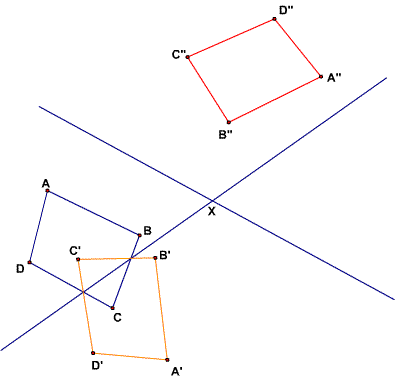
\includegraphics[scale=0.5]{2reflections}
\end{center}
What happens if we change the order of reflections?

\begin{mdsoln}
We will be using directed angles – i.e., all angles are read clockwise and taken modulo $ 180^\circ$.

Suppose we reflect point $ A$ about line $ \ell_1$ to give $ A'$ and then reflect $ A'$ about $ \ell_2$ to give $ A''$. Suppose that $ \ell_1$ and $ \ell_2$ meet at $ X$ and that $ P$ and $ Q$ are points on $ \ell_1$ and $ \ell_2$, respectively.

Observe that $ XA=XA'$ since $ X$ is on $ \ell_1$. Likewise, $ XA''=XA'=XA$. Now,\[ AXA''=\angle A'XA''-\angle A'XA=2\angle A'XQ-2\angle A'XP=2\angle PXQ\]Hence, $ A''$ is the image of $ A$ under a rotation of $ 2\angle PXQ$ (clockwise) about $ X$, which is what we wanted to prove.

If we were to change the order of reflections – i.e., reflect first about $ \ell_2$ and then about $ \ell_1$ - we would get a rotation about twice the other angle between $ \ell_1$ and $ \ell_2$. This would be the same rotation as we originally got, only in the other direction (i.e., counterclockwise instead of clockwise).    
\end{mdsoln}

\subsection{Problem 2}

Prove that the result of rotating a figure about two points, $ Y$, then $ Z$, through angles of $ y$ and $ z$, respectively, is equivalent to a rotation of $ y + z$ about $ X$, where $ X$ is the point such that $ ZYX = y/2$ and $ YZX = z/2$ (with the $ X$ chosen on the appropriate side of $ YZ$).

% https://s3.amazonaws.com/classroom.artofproblemsolving.com/Classes/GeomOlympiad/Images/2rotations.gif
\begin{center}
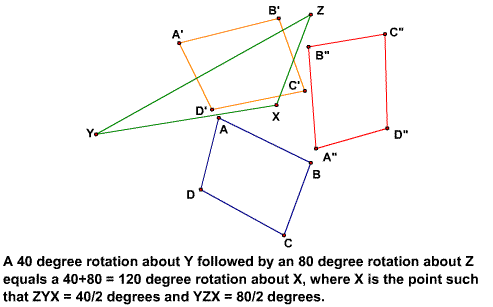
\includegraphics[scale=0.5]{2rotations}
\end{center}

\begin{mdsoln}
Let $ R_1$ denote a rotation of $ y$ about $ Y$ and $ R_2$ denote a rotation of $ z$ about $ Z$. Let $ T$ denote the transformation consisting of $ R_1$ followed by $ R_2$.

Observe that since $ \angle ZYX=y/2$, $ R_1$ takes $ X$ to the reflection $ X'$ of $ X$ over $ YZ$. Then, $ R_2$ takes $ X'$ back to $ X$. Hence, $ X$ is fixed under $ T$.

Let $ A$ be some point distinct from $ X$, with image $ A'$ under $ R_1$ and image $ A''$ under $ T$. We see that since $ T$ is composed of two rotations, it must preserve lengths; namely, $ AX$ must have the same length as its image $ A''X$ under $ T$. Moreover, the line $ AX$ must make an angle of $ y$ with its image $ A'X'$ under $ R_1$ and the line $ A'X'$ must make an angle of $ z$ with its image $ A''X$ under $ R_2$. Hence, $ AX$ must make an angle of $ y+z$ with $ A''X$. We conclude that $ A''$ must be the image of $ A$ under a rotation of $ y+z$ about $ X$, as desired.    
\end{mdsoln}

\subsection{Problem 3}

Squares $ BAXX'$ and $ CAYY'$ are constructed externally on the sides of isosceles triangle $ ABC$ ($ AB = AC$). Let $K$ be a variable point on side $BC$, and let $ E$ and $ F$ be the feet of the perpendiculars from $ K$ to $ CX$ and $ BY$, respectively, and let $ D$ be the midpoint of $ BC$.

a) Prove $ DE = DF$.

b) Find the locus of the midpoint of $ EF$.

% https://s3.amazonaws.com/classroom.artofproblemsolving.com/Classes/GeomOlympiad/Images/turkprob.gif
\begin{center}
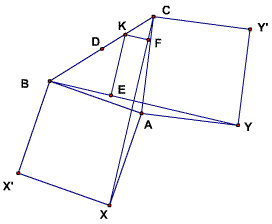
\includegraphics[scale=0.5]{turkprob}
\end{center}
\textit{Has hints.}
\begin{sketch}
    \begin{enumerate}
        \item Show that $ CX = BY$ and that the two segments are perpendicular.
        \item If you haven't tackled Hint 1, use a suitable rotation to prove it quickly.
        \item Let $ P$ be the intersection of $ CX$ and $ BY$. Prove that $ BPC$ is an isosceles right triangle.
        \item Prove that $ BDE$ and $ PDF$ are congruent triangles.
        \item What other segment is the midpoint of $ EF$ also the midpoint of?
    \end{enumerate}
\end{sketch}


\begin{mdsoln}
Note that $ \triangle BAY$ is the image of $ \triangle XAC$ under a rotation of $ 90^\circ$ about $ A$. Hence, if $ P$ is the intersection of $ CX$ and $ BY$, then $ \angle BPC=90^\circ$. By symmetry (about the line $ DA$), $ \triangle BPC$ is an isosceles triangle. Hence, it must be an isosceles right triangle.

Then, $ BD=PD$. Also, since $ KEPF$ is a rectangle, $ BE=BP-EP=CP-KF=CP-CF=PF$. Finally, $ \angle DBE=45^\circ=\angle DPF$. Hence, $ \triangle DBE\cong \triangle DPF$, so $ DE=DF$, as desired.

Note that the midpoint of $ EF$ is also the midpoint of $ KP$. The locus of this midpoint as $ K$ varies along segment $ BC$ is the image of $ BC$ under a dilation of ratio $ 1/2$ centered at $ P$. Hence, the desired locus is the segment connecting the midpoints of $ BP$ and $ CP$.    
\end{mdsoln}

\subsection{Problem 4}

On the sides $ AB$ and $ BC$ of triangle $ ABC$ we construct outward equilateral triangles with vertices $ D$ and $ E$. Show that the midpoints of $ AC$, $ BD$, and $ BE$ are vertices of an equilateral triangle.

% https://s3.amazonaws.com/classroom.artofproblemsolving.com/Classes/GeomOlympiad/Images/threeequil.gif

\begin{center}
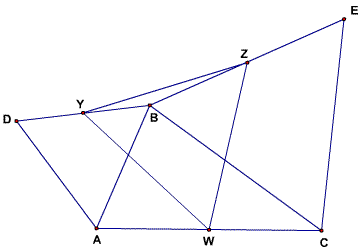
\includegraphics[scale=0.5]{threeequil}
\end{center}
\textit{Has hints.}
\begin{sketch}
    \begin{enumerate}
        \item Look at the points we have and decide which ones we want to be the centers of rotations and dilations. Should any new points be created?
        \item Construct a multi-part transformation, and show that it reduces to a simple rotation.
        \item Show that a 60-degree rotation of one of the points we want to show is on an equilateral triangle about one of the others is the third.
        \item Start with a dilation with ratio 2 and center B.
    \end{enumerate}
\end{sketch}


\begin{mdsoln}
Define the transformation $ T$ as follows: a dilation of ratio 2 about $ B$, then a rotation of $ 60^\circ$ (clockwise for the given diagram) about $ B$, and finally a dilation of ratio $ 1/2$ about $ A$, so that $ T$ takes point $ Z$ to point $ W$.

Observe that $ Y$ is a fixed point under $ T$ (since the component transformations defining $ T$ take $ Y$ to $ D$, then to the reflection $ A'$ of $ A$ over $ DB$, then back to $ Y$). It is evident also that $ T$ preserves lengths (since the component transformations defining $ T$ expand lengths by a factor of 2, then contract them again to their original size). Moreover, the image of a line under $ T$ makes an angle of $ 60^\circ$ (clockwise) with the original line (the component dilations defining $ T$ don’t affect this, since the image of line under a dilation is parallel to the original line).

Hence, $ YZ$ must have the same length as its image $ YW$ under $ T$, and must make angle of $ 60^\circ$ with it. Therefore, $ \triangle YZW$ must be equilateral, as desired.
    
\end{mdsoln}

\subsection{Problem 5}

In the diagram, $ ABC$ is equilateral. Point $ R$ is on $ AB$, $ P$ on $ BC$, and $ Q$ on $ AC$ such that $ ARQ$ and $ BRP$ are equilateral. Point $ N$ is constructed such that $ PQN$ is equilateral. Prove that $ NR$, $ BQ$, and $ AP$ are concurrent.

% https://s3.amazonaws.com/classroom.artofproblemsolving.com/Classes/GeomOlympiad/Images/brotconcur.gif
\begin{center}
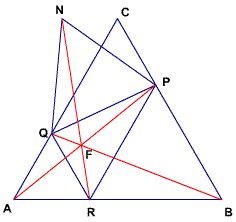
\includegraphics[scale=0.5]{brotconcur}
\end{center}
\textit{Has hints.}
\begin{sketch}
    \begin{enumerate}
        \item Are there any congruent triangles that we can rotate to each other?
        \item Angle chase!
        \item Find a cyclic quadrilateral.
    \end{enumerate}
\end{sketch}

\begin{mdsoln}
Let $ AP$ and $ BQ$ meet at $ F$. We want to show that $ NR$ goes through $ F$.

Observe that $ \triangle QRB$ is the image of $ \triangle ARP$ under a rotation of $ 60^\circ$ about $ R$. Hence, $ \angle BQR=\angle PAR$, so $ FQAR$ is cyclic, implying $ \angle RFQ=180^\circ-\angle QAR=120^\circ$. Likewise, $ FPBR$ is cyclic and $ \angle PFR=120^\circ$.

Hence, $ \angle QFP=120^\circ$, so $ NQFP$ is cyclic, implying that\[ \angle QFN=\angle QPN=60^\circ=180^\circ-\angle RFQ\]so $ F$ lies on $ NR$, as desired.
    
\end{mdsoln}
